%%%%%%%%%%%
%
% $Autor: Alexandra Roth $
% $Datum: today $
% $Pfad: Demontageanleitung.tex $
% $Version: 1.0 $
% !TeX spellcheck = de_DE
% !TeX encoding = utf8
% !TeX TXS-program:bibliography = txs:///biber
%
%%%%%%%%%%%%

\chapter{Demontageanleitung Heißdrahtschneidanlage \glqq ELMAR\grqq}


\section{Vorwort: Hinweise zur Demontage}

Die Demontage der Heißdrahtschneidanlage \glqq ELMAR\grqq{} ist ausschließlich auf sauberen, ebenen Flächen durchzuführen. Alle Werkzeuge, Hilfs- sowie Arbeitsmittel sollten vorab bereitliegen. Vor Beginn der Demontage ist die Anlage spannungsfrei zu schalten. Der Heißdraht, die Elektronik und das Netzteil müssen vollständig abgekühlt sein.

Ein Großteil der verbauten Komponenten stammt aus einem Creality Ender 5 Plus 3D-Drucker. Diese Teile sind im Folgenden entsprechend namentlich gekennzeichnet und können bei der Demontage sortiert aufbewahrt werden.

Die Demontage erfolgt grundsätzlich in umgekehrter Reihenfolge zur Montage. Dabei werden nur lösbare Schraub-, Steck- und Klemmverbindungen gelöst. Geklebte Verbindungen, aufgeklebte Aluminiumfolie, eingeschmolzene RUTHEX Gewinde-Einschmelzhülsen sowie eingepresste Lager werden nicht entfernt, sofern kein Austausch oder Defekt vorliegt.

Vor dem Trennen von elektrischen Steckverbindungen wird empfohlen, Fotos der Verkabelung anzufertigen und die Leitungen eindeutig zu markieren. Dadurch kann ein späterer Wiederaufbau leichter und fehlerärmer durchgeführt werden.

Schrauben, Muttern, Unterlegscheiben und Abstandselemente sollten nach Baugruppen getrennt gesammelt werden. Kleine Teile wie Nutensteine, Federn, Riemenrollen und Lagerbrücken sind gegen Verlust zu sichern.

Zur besseren Übersicht wurden Normteile (Schrauben, Muttern, Unterlegscheiben) teilweise ausgeblendet. Sie sind außerdem nur an den Stellen explizit genannt, an denen z.B. Verwechslungsgefahr besteht.

\textbf{ACHTUNG!} Der Heißdraht kann unter mechanischer Spannung stehen. Beim Lösen der Drahtspannung ist langsam und kontrolliert vorzugehen, damit der Draht nicht unkontrolliert zurückschnellt.

\section{Werkzeugauswahl}

Folgende Werkzeuge werden für die Demontage benötigt:

\begin{itemize}
	\item Innensechskantschlüssel-Satz
	\item Ringmaulschlüssel-Satz
	\item Schraubendreher
	\item Seitenschneider
	\item Spitzzange
	\item Schraubstock oder geeignete Ablage zum Fixieren einzelner Baugruppen
	\item Messschieber zur Kontrolle und Zuordnung von Bauteilen
\end{itemize}

Ein Lötkolben wird bei der normalen Demontage nicht benötigt, da eingeschmolzene RUTHEX Gewinde-Einschmelzhülsen nicht entfernt werden. Auch geklebte oder aufgeklebte Elemente werden nicht gelöst.

\section{Schritt 1: Vorbereitung und Sicherung der Anlage}

Vor der eigentlichen Demontage wird die Anlage vorbereitet und gesichert.

\begin{itemize}
	\item Anlage vollständig ausschalten und vom Netzteil trennen.
	\item USB-Verbindung zum Computer entfernen.
	\item Warten, bis Heißdraht, Netzteil, MOSFET und weitere elektronische Komponenten abgekühlt sind.
	\item Aktuellen Aufbau der Verkabelung fotografieren.
	\item Steckverbindungen, Endschalterleitungen, Motorleitungen und Leitungen des Heißdrahtes markieren.
	\item Schaumstoffreste, Schneidematte und lose Werkzeuge aus dem Arbeitsbereich entfernen.
\end{itemize}

\begin{figure}[htbp]
	\centering
	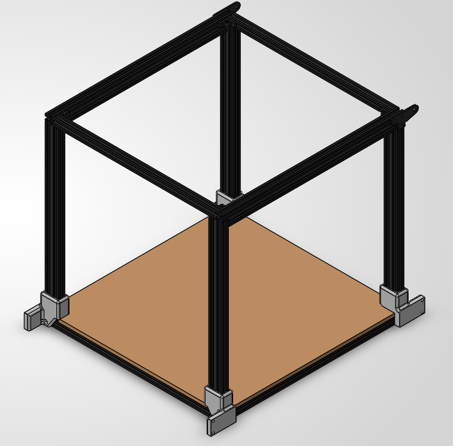
\includegraphics[width=0.65\textwidth]{General/ELMAR_CAD}
	\caption{Gesamtaufbau der Heißdrahtschneidanlage vor der Demontage}
	\label{fig:demontage_elmar_cad}
\end{figure}

\section{Schritt 2: Heißdraht entspannen und Abdeckkappe öffnen}

Zuerst wird die Spannung des Heißdrahtes reduziert, damit die folgenden Baugruppen gefahrlos gelöst werden können.

\begin{itemize}
	\item \glqq Druckteil Abdeckkappe\grqq{} vorsichtig öffnen.
	\item Einen Innensechskantschlüssel (5 mm) in die Aufnahme der \glqq Druckteil Drahtrolle\grqq{} einsetzen.
	\item Drahtrolle kontrolliert festhalten und die Federspannung langsam abbauen.
	\item Heißdraht auf der linken Seite an der Extruderdüse lösen und vorsichtig zurückführen.
	\item Heißdraht auf der \glqq Druckteil Drahtrolle\grqq{} sichern, damit er sich nicht unkontrolliert abwickelt.
\end{itemize}

\textbf{ACHTUNG!} Die aufgeklebte Aluminiumfolie auf der \glqq Druckteil Drahtrolle\grqq{} wird nicht entfernt. Sie bleibt auf dem Bauteil, da das Ablösen die Klebefläche oder das Druckteil beschädigen kann.

\begin{figure}[htbp]
	\centering
	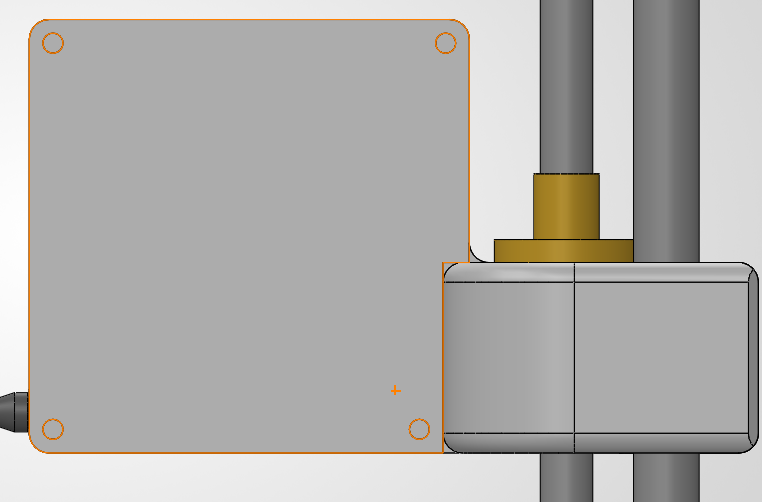
\includegraphics[width=0.55\textwidth]{General/Abdeckkappe}
	\caption{Abdeckkappe der Drahtrolle}
	\label{fig:demontage_abdeckkappe}
\end{figure}

\section{Schritt 3: Elektrik, Energieketten, Riemen und Schneidematte lösen}

In diesem Schritt werden die elektrischen und bewegungsführenden Komponenten gelöst, soweit dies ohne Beschädigung möglich ist.

\begin{itemize}
	\item Motorleitungen, Endschalterleitungen und Leitungen des Heißdrahtes anhand der zuvor erstellten Fotos trennen.
	\item Energieketten von den igus-Adaptern und Rahmenhaltern lösen.
	\item Riemenspannung über die Umlenkrolle reduzieren.
	\item Riemen aus der \glqq Creality Trägerplatte\grqq{} lösen und aus der Führung herausnehmen.
	\item Falls montiert, Schneidematte und lose Unterlagen entfernen.
	\item Stepper Motoren, Endschalter-Halter, Motorwinkel, Riemenrollen und Umlenkrollen abschrauben, sofern die Baugruppe vollständig zerlegt werden soll.
\end{itemize}

Die Bilder zeigen die linke Rahmenseite. Auf der rechten Seite ist ein hierzu symmetrischer Aufbau vorhanden.

\begin{figure}[htbp]
	\centering
	\begin{minipage}{0.48\textwidth}
		\centering
		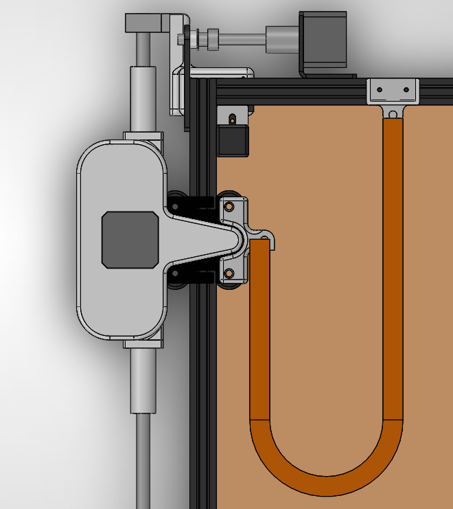
\includegraphics[width=\linewidth]{General/Rahmenseite_links}
		\caption{Rahmenseite links}
		\label{fig:demontage_rahmenseite_links}
	\end{minipage}
	\hfill
	\begin{minipage}{0.48\textwidth}
		\centering
		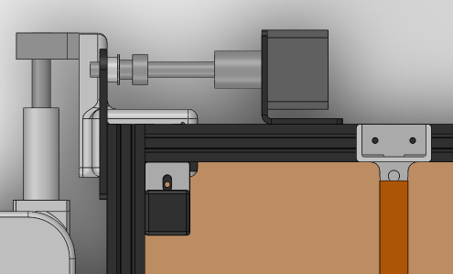
\includegraphics[width=\linewidth]{General/Rahmenseite_links_oben}
		\caption{Rahmenseite links, obere Ansicht}
		\label{fig:demontage_rahmenseite_links_oben}
	\end{minipage}
\end{figure}

\section{Schritt 4: Führung unten demontieren}

Nachdem Riemen und elektrische Leitungen gelöst sind, kann die untere Führung demontiert werden.

\begin{itemize}
	\item \glqq Creality Klemme für Führungsstab\grqq{} an \glqq Druckteil Eckhalter 1\grqq{} bzw. \glqq Druckteil Eckhalter 2\grqq{} lösen.
	\item \glqq Creality Führungsstahl horizontal\grqq{} vorsichtig aus den \glqq Creality Linearführungen rund\grqq{} herausziehen.
	\item Linearführungen und Klemmen sortiert ablegen.
	\item Darauf achten, dass die Vertikalwagen währenddessen nicht verkanten.
\end{itemize}

\section{Schritt 5: Horizontal- und Vertikalwagen aus dem Rahmen entnehmen}

Die beiden Baugruppen aus Horizontal- und Vertikalwagen können nun aus dem Grundrahmen entnommen werden.

\begin{itemize}
	\item Baugruppe von einer zweiten Person sichern lassen.
	\item \glqq Creality Rollen mit Lager\grqq{} oben am Rahmen entlasten.
	\item Baugruppe aus jeweils Horizontal- und Vertikalwagen vorsichtig oben aus dem Rahmen aushängen.
	\item Linke und rechte Seite getrennt markieren und ablegen, damit die Orientierung beim Wiederaufbau erhalten bleibt.
\end{itemize}

\begin{figure}[htbp]
	\centering
	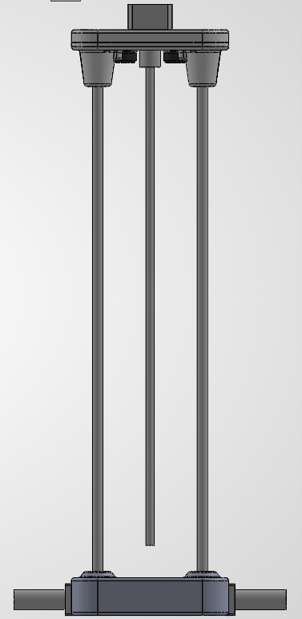
\includegraphics[width=0.55\textwidth]{General/Vertikalwagen_und_Horizontalwagen}
	\caption{Gefügter Vertikalwagen mit Horizontalwagen}
	\label{fig:demontage_vertikalwagen_und_horizontalwagen}
\end{figure}

\section{Schritt 6: Vertikalwagen von Horizontalwagen trennen}

Die Verbindung zwischen Vertikalwagen und Horizontalwagen wird gelöst, sofern die Baugruppen getrennt gelagert oder weiter zerlegt werden sollen.

\begin{itemize}
	\item Verschraubung der \glqq Creality Linearführung rund\grqq{} an \glqq Druckteil Führung unten\grqq{} lösen.
	\item \glqq Druckteil Führung unten\grqq{} abnehmen, sofern dies ohne Verkanten möglich ist.
	\item \glqq Unterbaugruppe Vertikalwagen links\grqq{} und \glqq Unterbaugruppe Vertikalwagen rechts\grqq{} vorsichtig von den Führungsstählen lösen.
	\item Eingeschmolzene RUTHEX M4 in \glqq Druckteil Führung unten\grqq{} nicht entfernen.
\end{itemize}

\section{Schritt 7: Unterbaugruppe Horizontalwagen demontieren}

Die Horizontalwagen werden nur so weit demontiert, wie es für Transport, Lagerung oder Austausch einzelner Teile sinnvoll ist.

\begin{itemize}
	\item \glqq Creality Kupplung\grqq{} und \glqq Creality Leitspindel TR8x2\grqq{} lösen.
	\item \glqq Creality Rollen mit Lager\grqq{}, \glqq Creality Abstandhülse für Rolle mit Lager\grqq{} und \glqq Exzentermutter\grqq{} demontieren.
	\item Stepper Motor abschrauben.
	\item \glqq Druckteil Endschalter-Halter rechts\grqq{} bzw. \glqq Druckteil Endschalter-Halter links\grqq{}, \glqq Creality Endschalter\grqq{} und \glqq Druckteil igus Adapter rechts\grqq{} bzw. \glqq Druckteil igus Adapter links\grqq{} lösen.
	\item Verschraubung von \glqq Druckteil Führung oben, Teil 1\grqq{} und \glqq Druckteil Führung oben, Teil 2\grqq{} nur lösen, wenn die Baugruppe vollständig zerlegt werden muss.
	\item \glqq Creality Führungsstahl vertikal\grqq{} nicht mit Gewalt aus dem Druckteil schlagen. Falls die Passung fest sitzt, verbleibt der Führungsstahl in der Baugruppe.
	\item Eingeschmolzene RUTHEX M3 und RUTHEX M5 bleiben im Druckteil.
\end{itemize}

\begin{figure}[htbp]
	\centering
	\begin{minipage}{0.32\textwidth}
		\centering
		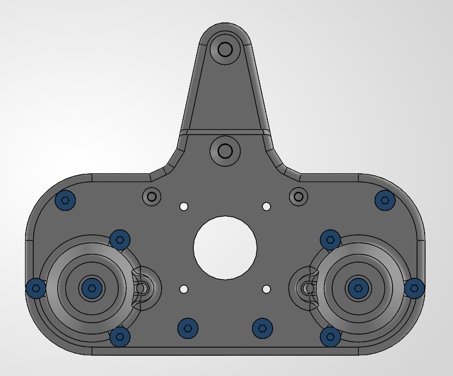
\includegraphics[width=\linewidth]{General/Horizontalwagen}
		\caption{Horizontalwagen}
		\label{fig:demontage_horizontalwagen}
	\end{minipage}
	\hfill
	\begin{minipage}{0.32\textwidth}
		\centering
		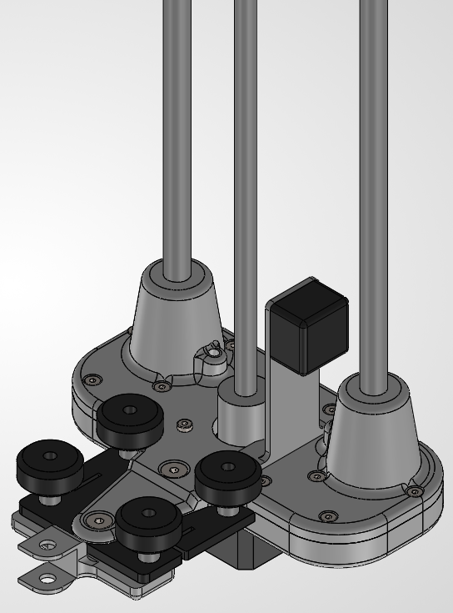
\includegraphics[width=\linewidth]{General/Horizontalwagen_montiert}
		\caption{Horizontalwagen montiert}
		\label{fig:demontage_horizontalwagen_montiert}
	\end{minipage}
	\hfill
	\begin{minipage}{0.32\textwidth}
		\centering
		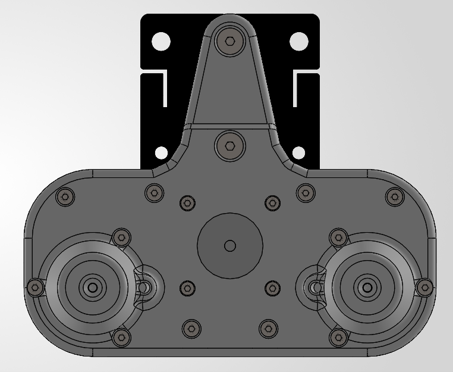
\includegraphics[width=\linewidth]{General/Horizontalwagen2}
		\caption{Horizontalwagen, weitere Ansicht}
		\label{fig:demontage_horizontalwagen_2}
	\end{minipage}
\end{figure}

\section{Schritt 8: Unterbaugruppe Vertikalwagen rechts demontieren}

Die Unterbaugruppe Vertikalwagen rechts enthält die Drahtrolle und wird daher vorsichtig und ohne Beschädigung des Heißdrahtes demontiert.

\begin{itemize}
	\item \glqq Druckteil Lagerbrücke\grqq{} abschrauben und zusammen mit dem vormontierten \glqq Rillenkugellager 12x21x5\grqq{} abnehmen.
	\item \glqq Druckteil Drahtrolle\grqq{} vorsichtig aus \glqq Druckteil Vertikalwagen rechts (Magazin)\grqq{} entnehmen.
	\item \glqq Flachspiralfeder\grqq{} entspannen und gesichert ablegen.
	\item Heißdraht auf der Rolle belassen oder separat aufwickeln, sofern er wiederverwendet werden soll.
	\item \glqq Extruderdüse 0.5 mm\grqq{} nur lösen, wenn sie gereinigt oder ersetzt werden soll.
	\item Eingepresste Rillenkugellager, Linearkugellager und eingeschmolzene RUTHEX Gewinde-Einschmelzhülsen nicht entfernen.
	\item Die aufgeklebte Aluminiumfolie auf der Drahtrolle nicht ablösen.
\end{itemize}

\begin{figure}[htbp]
	\centering
	\begin{minipage}{0.48\textwidth}
		\centering
		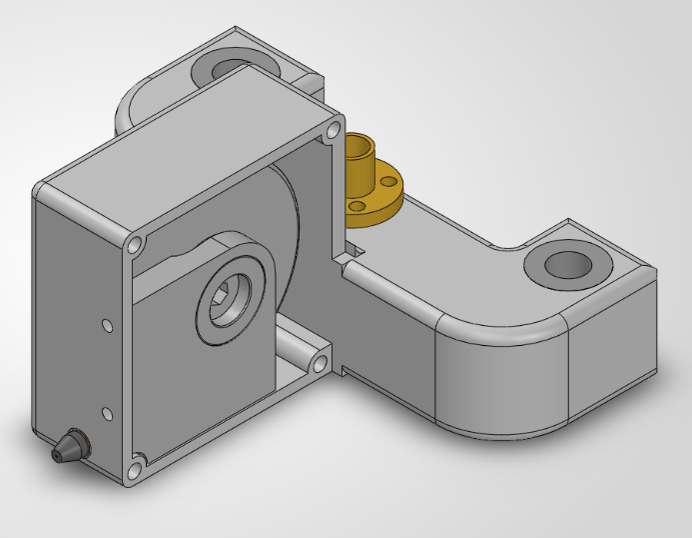
\includegraphics[width=\linewidth]{General/Vertikalwagen_rechts}
		\caption{Vertikalwagen rechts}
		\label{fig:demontage_vertikalwagen_rechts}
	\end{minipage}
	\hfill
	\begin{minipage}{0.48\textwidth}
		\centering
		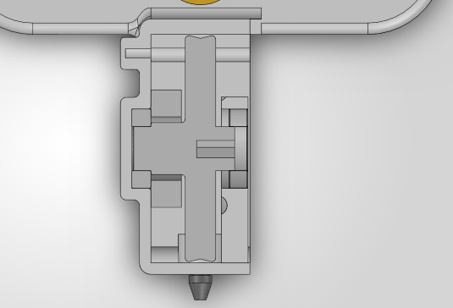
\includegraphics[width=\linewidth]{General/Vertikalwagen_rechts_unten}
		\caption{Vertikalwagen rechts, Unterseite}
		\label{fig:demontage_vertikalwagen_rechts_unten}
	\end{minipage}
\end{figure}

\section{Schritt 9: Unterbaugruppe Vertikalwagen links und Grundrahmen demontieren}

Zum Abschluss werden die linke Vertikalwagenbaugruppe und, falls erforderlich, der Grundrahmen zurückgebaut.

\begin{itemize}
	\item \glqq Extruderdüse 0.5 mm\grqq{} am linken Vertikalwagen nur lösen, wenn sie gereinigt oder ersetzt werden soll.
	\item \glqq Spindelmutter\grqq{} abschrauben, sofern der Vertikalwagen vollständig zerlegt werden muss.
	\item Eingepresste \glqq 64601006 Linearkugellager KB-3-ST Ø 10\grqq{} und eingeschmolzene RUTHEX M5 nicht entfernen.
	\item Holzplatte, Druckteil Eckhalter 1, Druckteil Eckhalter 2, Nutensteine und Nutenstein-Blöcke lösen, wenn der Grundrahmen zerlegt werden soll.
	\item Creality Aluminium-Extrusionsprofile, Bleche für Riemenrollen, Bleche für Umlenkrollen und Eckwinkel entsprechend der Ender-5-Plus-Rahmenmontage lösen.
	\item Geklebte oder verklebte Flächen nicht trennen. Bauteile mit Klebeverbindungen bleiben als Unterbaugruppe zusammen.
\end{itemize}

\begin{figure}[htbp]
	\centering
	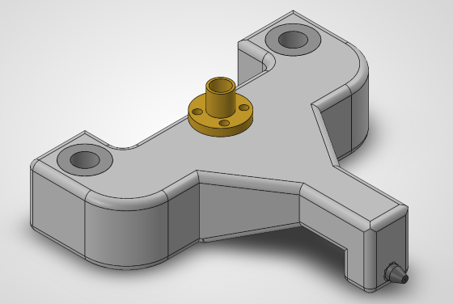
\includegraphics[width=0.58\textwidth]{General/Vertikalwagen_links}
	\caption{Unterbaugruppe Vertikalwagen links}
	\label{fig:demontage_vertikalwagen_links}
\end{figure}

Nach Abschluss der Demontage sind alle Bauteile trocken, sauber und nach Baugruppen sortiert zu lagern. Schrauben und Kleinteile sollten gemeinsam mit der jeweiligen Baugruppe verpackt werden, damit die Anlage bei Bedarf wieder montiert werden kann.
